\chapter{Teorema del Codice Sorgente e Compressione}

\section{Massimizzare l'informazione di una variabile aleatoria}

Come abbiamo visto nella sezione precedente, l'\textbf{Informazione di Shannon} e dell'\textbf{Entropia} di una variabile aleatoria X sono essenziali per misurare l'informazione ottenuta e l'incertezza rimanente. 

Ma come possiamo \textbf{massimizzare} l'informazione ottenuta da una variabile aleatoria? E quanti bit servono per descrivere il risultato di un esperimento?

L'ideale è ottenere una strategia che massimizzi l'informazione ottenuta nel caso medio ad ogni risultato ottenuto da una v.a. e stabilire un limite inferiore di tentativi da realizzare per ottenere l'informazione intera.
Definiamo:
\begin{itemize}
	\item Il \textbf{numero} di possibili risultati con $|A_X|$
	\item Assegnamo un nome \textbf{binario} ad ogni risultato
	\item Il \textbf{raw-bit content} di $X$, ovvero la \textbf{dimensione} di ogni nome, è: $$H_0 =\log_{2}|A_X|$$
	\item Il raw-bit content corrisponde ad un \textbf{limite inferiore} per individuare il risultato di $X$.
\end{itemize}
%
Spieghiamo meglio il concetto con degli esempi pratici.

\paragraph{Gioco del 63 (o del 64)}
Il gioco consiste nell'individuare un intero $x$ compreso tra 0 e 63 (o 1 e 64) nel numero \textbf{minore} di "SI" e "NO" possibile. Come possiamo fare?

Prima di individuare la strategia ottima, associamo alle risposte "SI" e "NO" i nomi binari $\{1, 0\}$ e calcoliamo l'\textbf{entropia} (raw-bit content). Sapendo che il numero di risultati è \textbf{equiprobabile} (distribuzione uniforme), l'entropia calcolata sarà \textbf{massima}:
$$
H(X) = \log_{2} |A_X| = \log_{2} 64 = 6 
$$

Suppniamo che l'intero $x$ da indovinare sia 35, una strategia ottima è quella di usare il modulo e le potenze del due:
\begin{enumerate}
	\item È l'intero $x \geq 32$? SI $\Rightarrow 1$
	\item È l'intero $x \mod{32} \geq 16$? NO $\Rightarrow 0$
	\item È l'intero $x \mod{16} \geq 8$? NO $\Rightarrow 0$
	\item È l'intero $x \mod{8} \geq 4$? NO $\Rightarrow 0$
	\item È l'intero $x \mod{4} \geq 2$? SI $\Rightarrow 1$
	\item È l'intero $x \mod{2} = 1$? SI $\Rightarrow 1$
\end{enumerate}

Formiamo il numero: \verb|100011| $\Rightarrow 35$

Questa strategia è coerente con l'Informazione di Shannon, in quanto ad ogni tentativo svolto otteniamo:
$$
h(x) = \log_{2} \frac{1}{\frac{1}{2}} = \log_{2} 2 = 1\ \text{bit}
$$
Ed essendo 6 i tentativi, al sesto tentativo abbiamo ottenuto 6 bit, ovvero l'entropia.

Abbiamo quindi visto che l'Informazione di Shannon ha senso se i risultati della variabile aleatoria hanno la stessa probabilità. Ma continua ad avere senso se le probabilità ad ogni risultato ottenuto \textbf{cambiano}? Vediamo un altro esempio.

\paragraph{Gioco del Sottomarino}
Nella battaglia navale, ogni giocatore nasconde una flotta di navi in un mare, rappresentato con una matrice $8\times8$. Ad ogni turno, un giocatore prova a colpire le navi dell'altro giocatore colpendo uno slot della matrice. Ci sono tre possibili risultati, \verb|'mancato'|, \verb|'colpito'|, \verb|'colpito e affondato'|.

Per rappresentare l'esempio, semplifichiamo il gioco, dove ogni giocatore ha una sola nave (un sottomarino) di grandezza di un singolo slot. Ci sono quindi solo due possibili risultati:
\begin{center}
	\verb|'colpito'|, che indichiamo con \verb|'Y'|\quad e \quad \verb|'mancato'|, che indichiamo con \verb|'N'|
\end{center}

Essendo $|A_X| = 64$, l'entropia è di 6 bit, come nel gioco precedente.

Tuttavia, rispetto al gioco del 63, nel gioco del Sottomarino non abbiamo una distribuzione di probabilità uniforme, infatti:

\begin{minipage}{0.33\textwidth}
	\begin{center}
		Le probabilità al \textbf{1° lancio} sono:
		$$
		P(Y) = \frac{1}{64} \quad;\quad P(N) = \frac{63}{64}
		$$
	\end{center}
\end{minipage}
\begin{minipage}{0.33\textwidth}
	\begin{center}
		Le probabilità al \textbf{2° lancio} sono:
		$$
		P(Y) = \frac{1}{63} \quad;\quad P(N) = \frac{62}{63}
		$$
	\end{center}
\end{minipage}
\begin{minipage}{0.33\textwidth}
	\begin{center}
		Le probabilità al \textbf{3° lancio} sono:
		$$
		P(Y) = \frac{1}{62} \quad;\quad P(N) = \frac{61}{62}
		$$
	\end{center}
\end{minipage}

E così via.\\ L'informazione di Shannon ottenuta al primo tentativo, se dovessimo essere fortunati e beccare il sottomarino, sarebbe di 6 bit, ma se invece dovessimo mancarlo sarebbe:
$$
h(x) = h_1(N) = \log_{2} \frac{64}{63} = 0,0227\ \text{bit}
$$
Se mancassimo anche il secondo tentativo, l'Informazione di Shannon ottenuta sarebbe:
$$
h_2(N) = \log_{2} \frac{63}{62} = 0,0230\ \text{bit} 
$$
Se mancassimo i primi 32 tentativi, il totale di Informazione di Shannon sarebbe:
$$
\log_{2}\frac{64}{63} + \log_{2} \frac{63}{62} + \cdots + \log_{2}\frac{33}{32} = 0,0227 + 0,0230 + \cdots + 0,0430 = 1\ \text{bit}  
$$

Perché 1 bit? Perché adesso sappiamo che il sottomarino non si trova in nessuno dei 32 slot provati, che corrispondono al primo tentativo del gioco del 63. Allo stesso modo, dopo 48 tentativi falliti avremo ottenuto in tutto 2 bit di informazione. Se al 49esimo tentativo dovessimo indovinare, otterremo:
$$
h_49(Y) = \log_{2} \frac{1}{\frac{1}{16}} = \log_{2} 16 = 4\ \text{bit}
$$ 
che sommati ai 2 bit trovati prima, equivalgono ai 6 bit dell'entropia.

Supponiamo il caso peggiore, ovvero che troviamo il sottomarino al 64esimo tentativo.\\ Otterremmo ogni bit così:
\begin{enumerate}
	\item Dopo i primi 32 tentativi otterremo il 1° bit.
	\item Dopo 48 tentativi otterremo il 2° bit.
	\item Dopo 56 tentativi otterremo il 3° bit.
	\item Dopo 60 tentativi otterremo il 4° bit.
	\item Dopo 62 tentativi otterremo il 5° bit.
	\item Dopo 63 tentativi otterremo il 6° bit. Rimarrà un singolo slot libero, che sarà la posizione del sottomarino.
\end{enumerate}

Possiamo affermare che l'Informazione di Shannon, indipendentemente dalla distribuzione di probabilità, continua ad avere senso per misurare l'informazione ricavata da un evento.

\newpage
\section{Introduzione alla compressione}
Adesso possiamo discutere di quanti bit sono \textbf{necessari} per descrivere il risultato di un evento sorgente.
Dimostrare che è possibile comprimere i dati da una particolare sorgente in un file a $L$ bit per simbolo e ricostruire i dati in maniera affidabile equivale a dimostrare che il contenuto di informazione media di quella sorgente è al più $L$ bit per simbolo.

Utilizzeremo le nozioni base del Teorema del Codice Sorgente per la \textbf{compressione di una sorgente}. Esistono \textbf{due modi} per comprimere una sorgente:
\begin{enumerate}
	\item \textbf{Compressione Lossy}: Questo tipo di compressione consente la \textbf{perdita di informazione} per comprimere il file sorgente. Un compressore lossy comprime quindi alcuni file ma ne \textbf{mappa altri alla stessa codifica}.\\ Denoteremo con $\delta$ la probabilità di fallimento del compressore lossy. Se $\delta$ può essere ridotto ad un valore molto basso, il compressore può rivelarsi utile.
	
	\item \textbf{Compressione Lossless}: Questo tipo di compressione \textbf{non consente alcun tipo di perdita di informazione}. Un compressore lossless mappa tutti i file a \textbf{codifiche diverse}, con la conseguenza che alcuni file potrebbero \textbf{ingrandirsi} invece che ridursi.\\
	Vogliamo quindi creare un compressore dove la probabilità che un file si ingradisca sia \textbf{molto bassa} e quella in cui si riduca sia \textbf{molto elevata}.
\end{enumerate}

\section{Compressione Lossy}
Come possiamo creare una strategia di compressione lossy?
Indipendentemente dal tipo di compressore che vogliamo costruire, abbiamo bisogno di conoscere le probabilità di ogni possibile risultato.

Supponiamo di voler comprimere un \textbf{file di testo} formato da caratteri ASCII di un alfabeto $A_X$.\\ In un generico testo in inglese o in italiano con molta probabilità ci sono caratteri \textbf{molto utilizzati} e altri invece \textbf{molto meno}, che quindi possono essere rimossi dall'alfabeto $A_X$ per creare un alfabeto ridotto $A_X'$.

Potremmo quindi calcolare il \textbf{raw-bit content} degli alfabeti $A_X$ e $A_X'$ per vedere quanto \textbf{spazio risparmiamo}. Più caratteri siamo disposti a rimuovere, più la probabilità $\delta$ aumenta.

\textbf{Esempio N.1 - Compressione Lossy di un Alfabeto $A_X$}

Supponiamo di avere un alfabeto $A_X$ formato da questi caratteri e le rispettive probabilità:
$$
A_X = \{\verb|a, b, c, d, e, f, g, h|\}\qquad\qquad P_X = \left\{\frac{1}{4}, \frac{1}{4}, \frac{1}{4}, \frac{3}{16}, \frac{1}{64}, \frac{1}{64}, \frac{1}{64}, \frac{1}{64}\right\}
$$

Calcoliamo il \textbf{raw-bit content} di $A_X$:
$$
H_0(X) = \log_{2} 8 = 3\ \text{bit}
$$

Vogliamo comprimere l'alfabeto $A_X$ eliminando i caratteri poco probabili, ovvero $\{\verb|e,f,g,h|\}$.

Abbiamo così un alfabeto $A_X'$ formato da $\{\verb|a,b,c,d|\}$, il cui raw-bit content è $H_0(X') = \log_2 4 = 2\ \text{bit}$ e un $\delta = \frac{1}{16}$.

Per formalizzare una strategia di compressione con un rischio $\delta$, creiamo il più piccolo insieme $S_\delta$ affinché la probabilità che $x$ non sia in $S_\delta$ è:

\begin{equation}
	Pr(x\notin S_\delta) \leq \delta
\end{equation}

\newpage
\subsection{Strumenti per la compressione lossy}
Definiamo due \textbf{strumenti fondamentali} per una compressione lossy ideale:
\begin{itemize}
	\item \textbf{Minimo insieme $\delta$-sufficiente}: Minimo sottoinsieme $S_\delta \subseteq A_X$ tale che:
	\begin{equation}
		Pr(x \in S_\delta) \geq 1 - \delta
	\end{equation}
	Questo sottoinsieme $S_\delta$ viene costruito in maniera greedy, ordinando gli elementi di $A_X$ in ordine decrescente in base alla loro probabilità ed aggiungendoli ad $S_\delta$ partendo da quelli più probabili, fino a quando la probabilità totale è $\geq 1 - \delta$. Possiamo infine assegnare un nome binario ad ogni elemento di $S_\delta$.
	
	\item \textbf{Essential bit content} di $X$ equivale a:
	\begin{equation}
		H_\delta(X) = \log_{2} |S_\delta|
	\end{equation}
	ed è la lunghezza delle codifiche di $S_\delta$.\\
	\textit{Osservazione}: Se $\delta=0$ l'essential bit content \textbf{coincide} con il raw-bit content.
\end{itemize}


\textbf{Esempio N.2 - Compressione lossy di blocchi di bit}

Supponiamo una variabile aleatoria $X$ che può assumere i valori
$x_i \in \{0,1\}$ con:
\begin{itemize}
	\item $Pr[x_i = 0] = p_0 = 0.9$
	\item $Pr[x_i = 1] = p_1 = 0.1$
\end{itemize}

Suppondendo una stringa di 4 bit, a quanto equivale l'\textbf{essential bit content} di questa stringa?

Prendiamo in considerazione \textbf{i casi possibili}:
\begin{enumerate}
	\item $Pr[X=0000]= p_0^4 = 0,6561$
	\item $P[X=\text{"x contiene un 1"}] = 4 \cdot (p_0^3\cdot p_1) = 4 \cdot 0,0729 = 0,3036$
	\item $P[X=\text{"x contiene due 1"}]= 6 \cdot (p_0^2 \cdot p_1^2) = 6\cdot 0,0081 = 0,0486$
	\item $P[X=\text{"x contiene tre 1"}]= 4 \cdot (p_0 \cdot p_1^3) = 4 \cdot 0,0009 = 0,0036$
	\item $P[X=1111]=0,00014$
\end{enumerate}

Essendo $A_X = 16$, calcolo il raw-bit content: $H_0(X) = \log_{2} 16 = 4\ \text{bit}$

Di conseguenza, per una compressione lossy efficace, potremmo sicuramente eliminare i casi 4 e 5 e mantenere i casi 1 e 2.
Abbiamo due opzioni con il caso 3:
\begin{itemize}
	\item Se lo mantenessimo, avremmo: 
	$$Pr[X= \text{"x contiene al massimo due 1"}] > 0,99$$ 
	e un $\delta = 0,01$. Sapendo quindi che $|S_\delta| = 11$ posso calcolare l'essential bit content:
	$$
	H_\delta(X^{11}) = \log_{2} 11 = 3,45\ \text{bit}
	$$
	Mantenendo il caso 3 ho risparmiato solamente 0,55 bit.
	
	\item Se lo rimuovessimo, avremmo:
	$$Pr[X= \text{"x contiene al massimo un 1"}] > 0,94$$ 
	e un $\delta = 0,06$. Sapendo quindi che $|S_\delta| = 5$ posso calcolare l'essential bit content:
	$$
	H_\delta(X^5) = \log_{2} 5 = 2,32\ \text{bit}
	$$
	Rimuovendo il caso 3 ho risparmiato 1,68 bit, un risparmio più consistente, con un $\delta$ sempre basso.
\end{itemize}

\newpage
Da questo esempio possiamo constatare che $H_\delta(X^N)$ \textbf{dipenda troppo} dal parametro $\delta$, un comportamento che dovremmo evitare. Questo tuttavia succede solo con un $N$ \textbf{piccolo} infatti, al crescere di $N$, $H_\delta(X^N)$ diventa sempre meno dipendente da $\delta$.

Possiamo quindi normalizzare rispetto alla lunghezza $N$ di una qualsiasi stringa binaria: $\frac{1}{N}H_\delta(x^N)$
\begin{minipage}{0.50\textwidth}
	\begin{figure}[H]
		\centering
		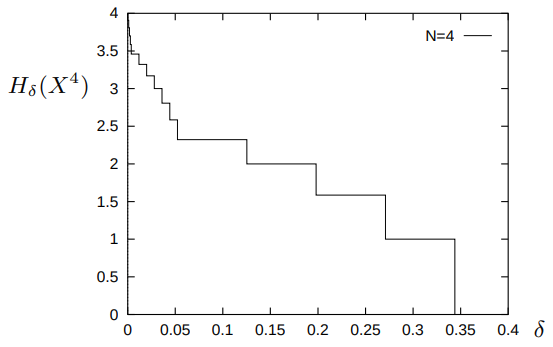
\includegraphics[width=0.9\textwidth]{images/lossy1.png}
	\end{figure}
\end{minipage}
\begin{minipage}{0.50\textwidth}
	\begin{figure}[H]
		\centering
		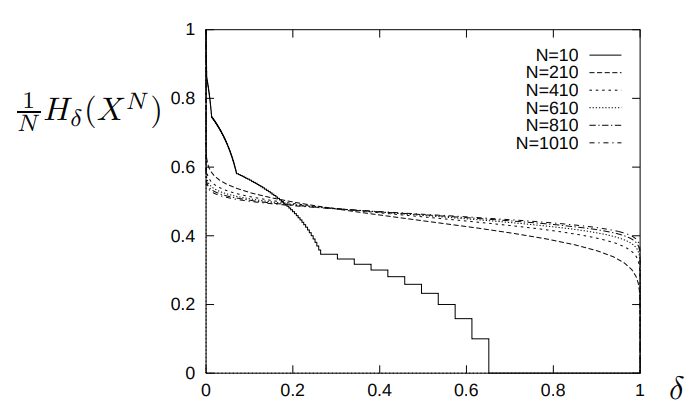
\includegraphics[width=1\textwidth]{images/lossy2.png}
	\end{figure}
\end{minipage}

Questo fenomeno è detto \textbf{Tipicalità}, cioè al crescere di $N$ la stringa più probabile aumenta il proprio peso e ci si avvicina al comportamento tipico.


\subsection{Teorema del Codice Sorgente di Shannon}
Data una variabile aleatoria $X$ con un'entropia $H(X) = H\ \text{bit}$, un $\varepsilon > 0$ e $0 < \delta < 1$ allora esiste $N_0 \in \mathbb{N}^+$ tale che, per $N > N_0$ vale:
\begin{equation}
	\left| \frac{1}{N} H_\delta(X^N)-H \right| < \varepsilon	
\end{equation}
Di conseguenza:
$$
H - \varepsilon < \frac{1}{N} H_\delta(X^N) < H + \varepsilon
$$

Da questo teorema possiamo dedurre due importanti risultati:
\begin{enumerate}
	\item Il primo deriva da: $$\frac{1}{N} H_\delta(X^N) < H + \varepsilon$$
	che afferma che anche per $\delta$ molto piccoli, il numero di bit per simbolo $\frac{1}{N} H_\delta(X^N)$ necessario per specificare una stringa $x$ con $N$ simboli con probabilità di errore bassa non deve eccedere gli $H + \varepsilon$ bit. Abbiamo bisogno di una \textbf{piccola tolleranza} per errore e il numero di bit richiesti crolla da $H_0(X)$ a $(H+\varepsilon)$. 
	
	\item Il secondo deriva da: $$H - \varepsilon < \frac{1}{N} H_\delta(X^N)$$
	che afferma che anche se il nostro compressore fosse molto tollerante agli errori di compressione, con un $\delta$ vicino a 1, il \textbf{numero medio} di bit per simbolo necessari per rappresentare $x$ devono essere almeno $H - \varepsilon$ bit.
\end{enumerate}

Questi due estremi quindi affermano che, indipendentemente dalla nostra tolleranza all'errore, il numero di bit per simbolo necessari per rappresentare $x$ è $H$ bit.

\newpage
\section{Compressione lossless}

A differenza della compressione lossy, dove i blocchi di codice avevano \textbf{lunghezza fissa} e venivano compressi con la \textbf{stessa codifica}, nella compressione lossless ogni file ha \textbf{lunghezza variabile} e per ogni file vengono usate \textbf{codifiche diverse} con la garanzia di comprimere e decomprimere \textbf{senza errori}.

L'idea è quella di poter comprimere, in media, assegnando codifiche \textbf{più brevi} a simboli/risultati \textbf{più probabili} e codifiche \textbf{più lunghe} a simboli/risultati \textbf{meno probabili}. Questo approccio non è tuttavia esente da difetti:
\begin{enumerate}
	\item Se alcuni codici simbolici sono accorciati, di quanto gli altri codici potrebbero essere allungati?
	\item Come possiamo assicurarci che un codice simbolico sia facile da decodificare?
	\item Come possiamo arrivare alla miglior compressione di un codice?
\end{enumerate}

\textbf{Notazione per gli alfabeti}
\begin{itemize}
	\item $A^N$ denota l'insieme delle N-tuple ordinate di elementi di $A$. Esempio:
	$$
	\{0,1\}^3 = \{000,001,010,011,100,101,110,111\}
	$$
	\item $A^*$ denota l'insieme delle stringhe di lunghezza finita su $A$. Esempio:
	$$
	\{0,1\}^* = \{0,1,00,01,10,11,000,001,\cdots\}
	$$
\end{itemize}

\subsection{Codici Simbolici}
\subsubsection{Definizioni di Codice Simbolico e Codice Esteso}
Un \textbf{codice simbolico} (binario) $C$ di una variabile aleatoria $X$ è una mappatura dei valori\\ $A_X = \{a_1, \cdots, a_n\} \rightarrow \{0,1\}^*$. Denotiamo con $c(x)$ ogni \textit{codeword} che corrisponde ad $x$ e con $l(x)$ denotiamo la \textbf{lunghezza} della codifica.

Il \textbf{codice esteso} può essere visto come una mappa da $A_X^* \rightarrow \{0,1\}^*$ ottenuto per \textbf{concatenazione} delle codeword corrispondenti (senza punteggiatura):
\begin{equation}
	c^*:A_X^*\rightarrow \{0,1\}^* \quad , \quad c^*(x_1 x_2 \cdots x_N) = c(x_1)c(x_2)\cdots c(x_N)
\end{equation}

Affinché un codice simbolico sia utile deve rispecchiare tre requisiti:
\begin{enumerate}
	\item Dev'essere \textbf{Univocamente Decodificabile}.
	\item Dev'essere facile da decodificare.
	\item Dev'essere compresso il più possibile.
\end{enumerate}

\subsubsection{Definizione di Codice Univocamente Decodificabile}
Un codice simbolico $x(X)$ è \textbf{univocamente decodificabile} se il corrispondente codice esteso $C^*(X)$ è tale che non esistano due stringhe distinte con la stessa codifica:
$$
\forall x,y \in A_X^*\ ,\ x \neq y \Rightarrow c^*(x) \neq c^*(y)
$$

\textbf{Esempio N.1 - Codice univocamente decodificabile}

Dato un codice simbolico per una variabile aleatoria $X$ definito in:\\
\begin{minipage}{0.50\textwidth}
	$$
	A_X = \{\verb|a, b, c, d|\}\qquad P_X = \left\{\frac{1}{2}, \frac{1}{4}, \frac{1}{8}, \frac{1}{8}
	\right\}
	$$
\end{minipage}
\begin{minipage}{0.50\textwidth}
	\begin{table}[H]
		\centering
		\begin{tabular}{c|cc}
			$a_i$ & $c(a_i)$ & $l_i$ \\
			\hline
			$a$ & 1000 & 4 \\
			$b$ & 0100 & 4 \\
			$c$ & 0010 & 4 \\
			$d$ & 0001 & 4 \\
		\end{tabular}
	\end{table}
\end{minipage}

Usando il codice esteso, potremmo codificare la stringa \verb|acdbac| come:
$$
c^*(\verb|acdbac|) = \verb|100000100001010010000010|.
$$
Questa codifica è \textbf{univocamente decodificabile}.

\newpage

\textit{OSSERVAZIONE}: Un codice simbolico è più semplice da decodificare se è possibile identificarne la fine di una codeword non appena essa si presenta, ciò significherebbe che \textbf{nessuna codeword può essere prefisso di un'altra}.

\subsection{Codici Prefix-free}
Una stringa $c$ è \textbf{prefisso} di un'altra $d$ se esiste una stringa-coda (o suffisso) $s$ tale che: $cs = d$.\\
Esempio: 1 e 10 sono entrambi prefisso di 101.

\subsubsection{Definizione di Codice Prefix-free}
Un codice simbolico è detto \textbf{Prefix-free} se nessuna codeword è prefisso di un'altra.
\begin{itemize}
	\item I codici prefix-free sono anche chiamati \textbf{istantanei} o \textbf{autopunteggiati}.
	\item I codici prefix-free sono \textbf{univocamente decodificabili}.
	\item I codici prefix-free sono associati a degli \textbf{alberi binari}, che possono essere incompleti se l'albero ha rami non utilizzati e completi se invece ogni ramo è usato.
\end{itemize}

\textbf{Esempio N.2 - Codici Prefix-free}

\begin{enumerate}
	\item Il codice $C_1 = \{0, 101\}$ è prefix-free e l'albero che forma è incompleto.
	\begin{center}
		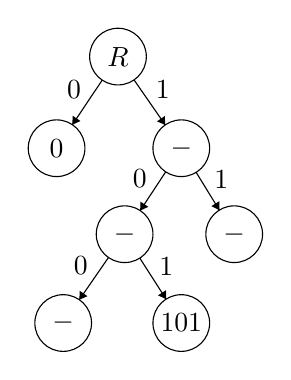
\begin{tikzpicture}[scale=0.12]
			\tikzstyle{every node}+=[inner sep=0pt]
			\draw [black] (37.4,-14.3) circle (3);
			\draw (37.4,-14.3) node {$R$};
			\draw [black] (30.9,-24) circle (3);
			\draw (30.9,-24) node {$0$};
			\draw [black] (44.1,-24) circle (3);
			\draw (44.1,-24) node {$-$};
			\draw [black] (49.7,-33.1) circle (3);
			\draw (49.7,-33.1) node {$-$};
			\draw [black] (38.1,-33.1) circle (3);
			\draw (38.1,-33.1) node {$-$};
			\draw [black] (31.6,-42.5) circle (3);
			\draw (31.6,-42.5) node {$-$};
			\draw [black] (44.1,-42.5) circle (3);
			\draw (44.1,-42.5) node {$101$};
			\draw [black] (35.73,-16.79) -- (32.57,-21.51);
			\fill [black] (32.57,-21.51) -- (33.43,-21.12) -- (32.6,-20.56);
			\draw (33.54,-17.81) node [left] {$0$};
			\draw [black] (39.1,-16.77) -- (42.4,-21.53);
			\fill [black] (42.4,-21.53) -- (42.35,-20.59) -- (41.53,-21.16);
			\draw (41.35,-17.79) node [right] {$1$};
			\draw [black] (45.67,-26.55) -- (48.13,-30.55);
			\fill [black] (48.13,-30.55) -- (48.13,-29.6) -- (47.28,-30.13);
			\draw (47.53,-27.27) node [right] {$1$};
			\draw [black] (42.45,-26.5) -- (39.75,-30.6);
			\fill [black] (39.75,-30.6) -- (40.61,-30.2) -- (39.77,-29.65);
			\draw (40.49,-27.22) node [left] {$0$};
			\draw [black] (36.39,-35.57) -- (33.31,-40.03);
			\fill [black] (33.31,-40.03) -- (34.17,-39.66) -- (33.35,-39.09);
			\draw (34.25,-36.44) node [left] {$0$};
			\draw [black] (39.71,-35.63) -- (42.49,-39.97);
			\fill [black] (42.49,-39.97) -- (42.48,-39.03) -- (41.63,-39.57);
			\draw (41.72,-36.49) node [right] {$1$};
		\end{tikzpicture}
	\end{center}
	
	\item Il codice $C_2 = \{1, 101\}$ \textbf{non è} prefix-free, tuttavia è univocamente decodificabile.
	
	\item Il codice $C_3 = \{0, 10, 110, 111\}$ è prefix-free e l'albero che forma è completo.
	\begin{center}
		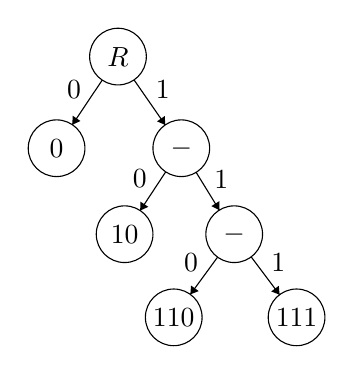
\begin{tikzpicture}[scale=0.12]
			\tikzstyle{every node}+=[inner sep=0pt]
			\draw [black] (37.4,-14.3) circle (3);
			\draw (37.4,-14.3) node {$R$};
			\draw [black] (30.9,-24) circle (3);
			\draw (30.9,-24) node {$0$};
			\draw [black] (44.1,-24) circle (3);
			\draw (44.1,-24) node {$-$};
			\draw [black] (49.7,-33.1) circle (3);
			\draw (49.7,-33.1) node {$-$};
			\draw [black] (38.1,-33.1) circle (3);
			\draw (38.1,-33.1) node {$10$};
			\draw [black] (56.3,-41.9) circle (3);
			\draw (56.3,-41.9) node {$111$};
			\draw [black] (43.3,-41.9) circle (3);
			\draw (43.3,-41.9) node {$110$};
			\draw [black] (35.73,-16.79) -- (32.57,-21.51);
			\fill [black] (32.57,-21.51) -- (33.43,-21.12) -- (32.6,-20.56);
			\draw (33.54,-17.81) node [left] {$0$};
			\draw [black] (39.1,-16.77) -- (42.4,-21.53);
			\fill [black] (42.4,-21.53) -- (42.35,-20.59) -- (41.53,-21.16);
			\draw (41.35,-17.79) node [right] {$1$};
			\draw [black] (45.67,-26.55) -- (48.13,-30.55);
			\fill [black] (48.13,-30.55) -- (48.13,-29.6) -- (47.28,-30.13);
			\draw (47.53,-27.27) node [right] {$1$};
			\draw [black] (42.45,-26.5) -- (39.75,-30.6);
			\fill [black] (39.75,-30.6) -- (40.61,-30.2) -- (39.77,-29.65);
			\draw (40.49,-27.22) node [left] {$0$};
			\draw [black] (51.5,-35.5) -- (54.5,-39.5);
			\fill [black] (54.5,-39.5) -- (54.42,-38.56) -- (53.62,-39.16);
			\draw (53.58,-36.1) node [right] {$1$};
			\draw [black] (47.94,-35.53) -- (45.06,-39.47);
			\fill [black] (45.06,-39.47) -- (45.94,-39.12) -- (45.13,-38.53);
			\draw (45.91,-36.12) node [left] {$0$};
		\end{tikzpicture}
	\end{center}
	
	\item Il codice $C_4 = \{00, 01, 10, 11\}$ è prefix-free e l'albero che forma è completo.
	\begin{center}
		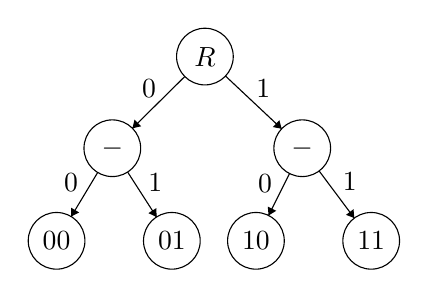
\begin{tikzpicture}[scale=0.12]
			\tikzstyle{every node}+=[inner sep=0pt]
			\draw [black] (37.4,-14.3) circle (3);
			\draw (37.4,-14.3) node {$R$};
			\draw [black] (27.6,-24) circle (3);
			\draw (27.6,-24) node {$-$};
			\draw [black] (47.7,-24) circle (3);
			\draw (47.7,-24) node {$-$};
			\draw [black] (55,-33.8) circle (3);
			\draw (55,-33.8) node {$11$};
			\draw [black] (42.8,-33.8) circle (3);
			\draw (42.8,-33.8) node {$10$};
			\draw [black] (33.9,-33.8) circle (3);
			\draw (33.9,-33.8) node {$01$};
			\draw [black] (21.7,-33.8) circle (3);
			\draw (21.7,-33.8) node {$00$};
			\draw [black] (35.27,-16.41) -- (29.73,-21.89);
			\fill [black] (29.73,-21.89) -- (30.65,-21.68) -- (29.95,-20.97);
			\draw (31.48,-18.67) node [above] {$0$};
			\draw [black] (39.58,-16.36) -- (45.52,-21.94);
			\fill [black] (45.52,-21.94) -- (45.28,-21.03) -- (44.59,-21.76);
			\draw (43.57,-18.67) node [above] {$1$};
			\draw [black] (49.49,-26.41) -- (53.21,-31.39);
			\fill [black] (53.21,-31.39) -- (53.13,-30.45) -- (52.33,-31.05);
			\draw (51.93,-27.51) node [right] {$1$};
			\draw [black] (46.36,-26.68) -- (44.14,-31.12);
			\fill [black] (44.14,-31.12) -- (44.95,-30.62) -- (44.05,-30.18);
			\draw (44.55,-27.79) node [left] {$0$};
			\draw [black] (29.22,-26.52) -- (32.28,-31.28);
			\fill [black] (32.28,-31.28) -- (32.27,-30.33) -- (31.42,-30.87);
			\draw (31.37,-27.59) node [right] {$1$};
			\draw [black] (26.05,-26.57) -- (23.25,-31.23);
			\fill [black] (23.25,-31.23) -- (24.09,-30.8) -- (23.23,-30.29);
			\draw (24.01,-27.63) node [left] {$0$};
		\end{tikzpicture}
	\end{center}
\end{enumerate}

\subsubsection{Definizione di Lunghezza Attesa}
La lunghezza attesa $L(C, X)$ di un codice simbolico $C$ per una variabile aleatoria $X$ è:
\begin{equation}
	L(C,X) = \sum_{x\in A_X} P(x)\cdot l(x) = \sum_{i=1}^{I} p_i\cdot l_i \qquad \text{dove}\ I = |A_X|
\end{equation}

\textbf{Esempio N.3 - Entropia e Lunghezza Attesa di un codice prefix-free}

Dato il codice simbolico $C_3$ (del precedente esempio) per una variabile aleatoria $X$ definito in:\\
\begin{minipage}{0.50\textwidth}
	$$
	A_X = \{\verb|a, b, c, d|\}\qquad P_X = \left\{\frac{1}{2}, \frac{1}{4}, \frac{1}{8}, \frac{1}{8}
	\right\}
	$$
\end{minipage}
\begin{minipage}{0.50\textwidth}
	\begin{table}[H]
		\centering
		\renewcommand{\arraystretch}{1.5}
		\begin{tabular}{c|c|c|c|c}
			$a_i$ & $c(a_i)$ & $p_i$ & $h(p_i)$ & $l(a_i)$ \\
			\hline
			$a$ & 0 & $\frac{1}{2}$ & 1 & 1 \\
			$b$ & 10 & $\frac{1}{4}$ & 2 & 2 \\
			$c$ & 110 & $\frac{1}{8}$ & 3 & 3 \\
			$d$ & 111 & $\frac{1}{8}$ & 3 & 3 \\
		\end{tabular}
	\end{table}
\end{minipage}

Calcoliamo l'entropia e la lunghezza attesa.
$$
H(X) = \frac{1}{2} \log_2 2+ \frac{1}{4} \log_2 4+ \frac{1}{8} \log_2 8+ \frac{1}{8} \log_2 8 = \frac{1}{2} + 2 \cdot \frac{1}{4} + 3 \cdot \frac{1}{4} = 1 + \frac{3}{4} = 1.75\ \text{bit}
$$
$$
L(C_3, X) = \frac{1}{2} \cdot 1 + \frac{1}{4} \cdot 2 + \frac{1}{8} \cdot 3 + \frac{1}{8} \cdot 3 = 1 + \frac{3}{4} = 1.75\ \text{bit}
$$

Il codice $C_3$ è prefix-free e $L(C_3, X) = H(X)$

\textbf{Esempio N.4 - Entropia e Lunghezza attesa di un codice non univocamente decodificabile}

Dato il codice simbolico $C_5 = \{0, 1, 10, 11\}$ per una variabile aleatoria $X$ definito in:\\
\begin{minipage}{0.50\textwidth}
	$$
	A_X = \{\verb|a, b, c, d|\}\qquad P_X = \left\{\frac{1}{2}, \frac{1}{4}, \frac{1}{8}, \frac{1}{8}
	\right\}
	$$
\end{minipage}
\begin{minipage}{0.50\textwidth}
	\begin{table}[H]
		\centering
		\renewcommand{\arraystretch}{1.5}
		\begin{tabular}{c|c|c|c|c}
			$a_i$ & $c(a_i)$ & $p_i$ & $h(p_i)$ & $l(a_i)$ \\
			\hline
			$a$ & 0 & $\frac{1}{2}$ & 1 & 1 \\
			$b$ & 1 & $\frac{1}{4}$ & 2 & 1 \\
			$c$ & 10 & $\frac{1}{8}$ & 3 & 2 \\
			$d$ & 11 & $\frac{1}{8}$ & 3 & 2 \\
		\end{tabular}
	\end{table}
\end{minipage}

Calcoliamo l'entropia e la lunghezza attesa.
$$
H(X) = 1.75\ \text{bit} \quad  L(C_5, X) = \frac{1}{2} \cdot 1 + \frac{1}{4} \cdot 2 + \frac{1}{8} \cdot 2 + \frac{1}{8} \cdot 2 = \frac{1}{2} + \frac{3}{4} = 1.25\ \text{bit}
$$

Il codice $C_5$ non solo non è prefix-free, ma non è nemmeno univocamente decodificabile e \\$L(C_5, X) < H(X)$

\textbf{Esempio N.5 - Entropia e Lunghezza attesa di un codice non prefix-free}

Dato il codice simbolico $C_6 = \{0, 01, 011, 111\}$ per una variabile aleatoria $X$ definito in:\\
\begin{minipage}{0.50\textwidth}
	$$
	A_X = \{\verb|a, b, c, d|\}\qquad P_X = \left\{\frac{1}{2}, \frac{1}{4}, \frac{1}{8}, \frac{1}{8}
	\right\}
	$$
\end{minipage}
\begin{minipage}{0.50\textwidth}
	\begin{table}[H]
		\centering
		\renewcommand{\arraystretch}{1.55}
		\begin{tabular}{c|c|c|c|c}
			$a_i$ & $c(a_i)$ & $p_i$ & $h(p_i)$ & $l(a_i)$ \\
			\hline
			$a$ & 0 & $\frac{1}{2}$ & 1 & 1 \\
			$b$ & 01 & $\frac{1}{4}$ & 2 & 2 \\
			$c$ & 011 & $\frac{1}{8}$ & 3 & 3 \\
			$d$ & 111 & $\frac{1}{8}$ & 3 & 3 \\
		\end{tabular}
	\end{table}
\end{minipage}

Calcoliamo l'entropia e la lunghezza attesa.
$$
H(X) = 1.75\ \text{bit} \quad  L(C_6, X) = \frac{1}{2} \cdot 1 + \frac{1}{4} \cdot 2 + \frac{1}{8} \cdot 3 + \frac{1}{8} \cdot 3 = 1 + \frac{3}{4} = 1.75\ \text{bit}
$$

Il codice $C_6$ non è prefix-free ma univocamente decodificabile e $L(C_6, X) = H(X)$.

Ma quali sono i limiti imposti dall'univoca decodificabilità?\\ Data una lista di interi $\{l_i\}$, esiste un codice univocamente decodificabile con lunghezze $l_i$?

Possiamo rispondere a queste domande grazie alla \textbf{Disuguaglianza di Kraft}

\newpage

\subsection{Disuguaglianza di Kraft}
\subsubsection{Definizione di Disuguaglianza di Kraft}
Per ogni codice univocamente decodificabile $C(X)$ sull'alfabeto binario $\{0,1\}$, le lunghezze delle codeword devono soddisfare:
\begin{equation}
	\sum_{i=1}^{I} 2^{-l_i} \leq 1 \qquad \text{dove}\ I = |A_X| 
\end{equation}

Se un codice univocamente decodificabile soddisfa la Disuguaglianza di Kraft con \textbf{uguaglianza}, allora si dice che quel codice è \textbf{completo}.

\textbf{Dimostrazione}

Definiamo $\sum_{i=1}^{I} 2^{l_i}$ e sia:
$$
S^N = \left[\sum_{i=1}^{I} 2^{l_i}\right]^N = \sum_{i_1 = 1}^{I} \sum_{i_2 = 1}^{I} \cdots \sum_{i_N = 1}^{I} 2^{-(l_{i_1} + l_{i_2} + \cdots l_{i_N})}
$$

La quantità dell'esponente, $(l_{i_1} + l_{i_2} + \cdots l_{i_N})$ è la lunghezza della codifica di una stringa $x = a_{i_1}\ a_{i_2}\cdots a_{i_N}$ e, per ognuna di tali stringhe, c'è un termine di questa somma.\\
Introduciamo un array $A_l$ che conta quante stringhe $x$ hanno lunghezza $l$.\\ Successivamente definiamo $l_{min} = min_i\cdot l_i$ e $l_{max} = max_i \cdot l_i$ tali che:
$$
S^N = \sum_{l=N\cdot l_{min}}^{N\cdot l_{max}} 2^{-l} A_l
$$

Poiché il codice C è univocamente decodificabile le codeword sono \textbf{tutte distinte} e quindi ci sono al più $2^l$ stringhe di lunghezza $l$, con $$A_l \leq 2^l$$

Allora:
$$
S^N = \sum_{l=N\cdot l_{min}}^{N\cdot l_{max}} 2^{-l} A_l \leq \sum_{l=N\cdot l_{min}}^{N\cdot l_{max}} 1 \leq N \cdot l_{max} \quad ,\ \forall N
$$

Se $S$ fosse $>1$ allora: $$S^N \leq N \cdot l_{max}$$
il ché è un assurdo, in quando $S^N$ ha crescita esponenziale mentre $N \cdot l_{max}$ crescita polinomiale.

\subsubsection{Disuguaglianza di Kraft per codici Prefix-free}
Dato un insieme di lunghezze che soddisfano:
$$
\sum_{i=1}^{I} 2^{-l_i} \leq 1
$$
esiste un codice prefix-free con queste lunghezze delle codeword.

\textbf{Dimostrazione}

Usiamo una strategia greedy. Date le lunghezze $l_1 \leq l_2 \leq \cdots \leq l_I$ consideriamo un albero binario con profondità $l_n = l_{max}$ e $2^{l_max}$ foglie. Diremo che un nodo al livello $l$ è disponbile se non è ancora stato scelto né è un discendente di un nodo scelto.

Al passo $i$:
\begin{itemize}
	\item Consideriamo un nodo $v$ con profondità $\leq l_i$. Se ha profondità $< l_i$, espandiamolo aggiungendo i suoi figli. Ripetiamo finché non arriviamo a profondità $l_i$
	\item Assegnamo $v$ come i-esima codeword. $v$ e i suoi discendenti non sono più disponibili.
\end{itemize}

Dopo aver assegnato le prime $i-1$ parole, il peso dei nodi disponibili è:
$$
W_i = \sum_{v} 2^{-depth(v)}\quad\text{con}\ v\ \text{disponibili}  
$$

\newpage

Affermo che $W_i \geq 2^{l_i}\ \forall i$ e pertanto al passo $i$ esiste almeno un nodo utilizzabile. Dimostriamo questa affermazione per induzione.

\textbf{Caso Base}: All'inizio l'unico nodo disponibile è la radice:
$$
W_1 = 2^0 = 1 \geq 2^{l_1}\quad,\ l_1 \geq 1
$$

\textbf{Passo Induttivo}: Supponiamo che l'affermazione sia vero fino al all'($i-1$)-esimo passo.

Al passo $i$, scegliamo un nodo $v$ a profondità $l_i$, che contribuisce con $2^{-l_i}$ al peso. Quindi:
$$
W_{i+1} = W_i - 2^{-l_i}
$$

Vogliamo $$W_{i+1} \geq 2^{-l_{i+1}}$$

Dalla diseguaglianza di Kraft applicata a tutti gli $n$ termini
$$
\sum_{j=1}^{n} 2^{-l_j} \leq 1 = W_1	\quad \text{e} \quad W_i = W_1 - \sum_{j=1}^{i-1} 2^{-l_j}
$$
quindi
$$
W_{i+1} = W_1 - \sum_{j=1}^{i} 2^{-l_j} \geq \sum_{j=i+1}^{n} 2^{-l_j} \geq 2^{-l_{i+1}}
$$

\subsection{Quanto possiamo comprimere una sorgente?}
\subsubsection{Limite inferiore	della lunghezza attesa}
La lunghezza $L(C,X)$ di un codice $C$ univocamente decodificabile è: 
\begin{equation}
	L(C,X) \geq H(X)
\end{equation}

\textbf{Dimostrazione}:

Definiamo le \textit{probabilità implicite}: 
$$
q_i = \frac{2^{-l_i}}{z}\quad \text{con} \quad z=\sum_{i} 2^{-l_i}
$$
affinché: 
$$
l_i = \frac{\log_{2} 1}{q_i - \log_{2} z}
$$
Usiamo quindi la diseguaglianza di Gibbs, per cui diventa:
$$
\sum_{i} p_i \log_{2} \frac{1}{q_i} \geq \sum_{i} p_i \log_2 \frac{1}{p_i}\quad \text{e vale se}\ q_i = p_i
$$
Infine con la diseguaglianza di Kraft con $z \leq 1$:
$$
L(C,X) = \sum_{i} p_i\cdot l_i = \sum_{i} p_i (\log_{2}\frac{1}{q_i} - \log_2 z) \geq \sum_{i} p_i (\log_{2}\frac{1}{p_i} - \log_2 z) \geq H(X)
$$

\subsubsection{Codice simbolico ottimo}
Se la lunghezza attesa è minimizzata ed è uguale all'entropia solo se le lunghezze delle codeword sono uguali all'Informazione di Shannon:
$$
l_i = \log_{2}\frac{1}{p_i}\quad \text{allora}\quad L(C,X)= H(X)
$$

\newpage
\subsubsection{Teorema del Codice Sorgente per Codici Simbolici}
Data una variabile aleatoria $X$ esiste un codice prefix-free $C$ la cui lunghezza attesa soddisfa:
\begin{equation}
	H(X) \leq L(C,X) \leq H(X) + 1
\end{equation}

\textbf{Dimostrazione}:

Arrotondiamo per \textbf{eccesso} le lunghezze delle codeword rispetto alla loro lunghezza \textbf{ottimale}: $$l_i = \ceil{\log_{2}\left(\frac{1}{p_i}\right)}$$
Controlliamo che la diseguaglianza di Kraft sia soddisfatta:
$$
\sum_{i=1}^{I} 2^{-l_i} = \sum_{i=1}^{I} 2^{-\ceil{\log_{2}(\frac{1}{p_i})}} \leq \sum_{i=1}^{I} 2^{-\log_{2}\frac{1}{p_i}} \leq \sum_{i=1}^{I} p_i = 1
$$
Calcoliamo:
$$
H(X) \leq L(C,X) = \sum_{i=1}^{I} p_i l_1 = \sum_{i=1}^{I} p_i \ceil{\log_{2}\frac{1}{p_i}} < \sum_{i} p_i (\log_{2} \frac{1}{p_i} + 1) = H(X) + 1
$$

\textit{OSSERVAZIONE}: Se usiamo un codice le cui probabilità sono $\{p_i\}_{i=1}^I$ e usiamo un codice completo con lunghezze $l_i$, esse ci definiscono le probabilità di un codice ottimale $q_i = 2^{-l_i}$.\\
La loro lunghezza attesa sarà:
$$
L(C,X) = H(X) + \sum_{i} p_i \log_{2}\frac{p_i}{q_i}
$$
con $\sum_{i} p_i \log_{2}\frac{p_i}{q_i}$ = $D_{KL}(P||Q)$ (Divergenza di Kullback-Leibler)

\newpage

\subsection{Codifica di Huffman}
\subsubsection{Procedura dell'algoritmo}
Dato un set di probabilità $P_X$, come possiamo trovare un codice prefix-free ottimo?\\
La codifica di Huffman costruisce un codice prefix-free ottimo che costruisce un \textbf{albero binario} dalle sue \textbf{foglie}.

\begin{enumerate}
	\item Si considerano i due simboli meno probabili dell'alfabeto $A_X$. A questi simboli assegniamo le codeword più lunghe, che avranno \textbf{stessa lunghezza} e differiranno soltanto per l'ultima cifra.	
	\item Combiniamo questi due simboli in un unico simbolo (che ha la somma delle probabilità degli stessi) e ripetiamo.
\end{enumerate}

Visto che ogni passo dell'algoritmo riduce la grandezza dell'alfabeto di uno, esso impiegherà $|A_X|-1$ passi.

\textbf{Esempio N.6 - Codifica di Huffman}

Supponiamo di avere una variabile aleatoria $X$ con:
$$
A_X = \{\verb|a, b, c, d, e|\}\qquad P_X = \left\{0.25,\ 0.25,\ 0.2,\ 0.15,\ 0.15 \right\}
$$
\begin{minipage}{0.50\textwidth}
	\begin{figure}[H]
		\centering
		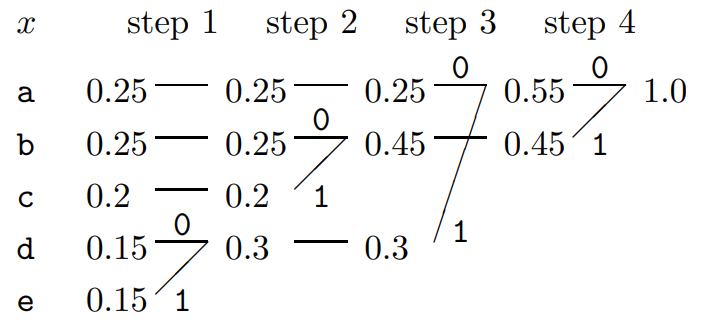
\includegraphics[width=1\textwidth]{images/huffman.png}
	\end{figure}
\end{minipage}
\begin{minipage}{0.50\textwidth}
	\begin{table}[H]
		\centering
		\renewcommand{\arraystretch}{1.55}
		\begin{tabular}{c|c|c|c|c}
			\hline
			$a_i$ & $p_i$ & $h(p_i)$ & $l_i$ & $c(a_i)$ \\
			\hline
			$a$ & 0.25 & 2.0 & 2 & 00 \\
			$b$ & 0.25 & 2.0 & 2 & 10 \\
			$c$ & 0.2 & 2.3 & 2 & 11 \\
			$d$ & 0.15 & 2.7 & 3 & 010 \\
			$d$ & 0.15 & 2.7 & 3 & 011 \\
			\hline
		\end{tabular}
	\end{table}
\end{minipage}

Calcoliamo l'entropia $H(X)$ e la lunghezza attesa $L(C,X)$
$$
H(X) = \frac{1}{4} \log_{2} 4 + \frac{1}{4} \log_{2} 4 + \frac{1}{5} \log_{2} 5 + \frac{3}{20} \log_{2} \frac{20}{3} + \frac{3}{20} \log_{2} \frac{20}{3} \approx 2,2855\ \text{bit}
$$
$$
L(C,X) = \frac{1}{4} \cdot 2 + \frac{1}{4} \cdot 2 + \frac{1}{5} \cdot 2 + \frac{3}{20} \cdot 3 +\frac{3}{20} \cdot 3 = 1 + \frac{2}{5} + \frac{9}{10} = \frac{23}{10} = 2,3\ \text{bit}
$$

\begin{center}
	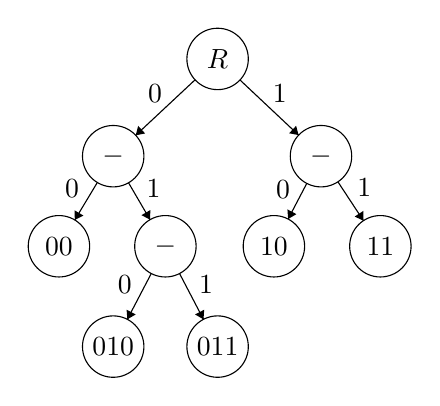
\begin{tikzpicture}[scale=0.13]
		\tikzstyle{every node}+=[inner sep=0pt]
		\draw [black] (37.9,-10.4) circle (3);
		\draw (37.9,-10.4) node {$R$};
		\draw [black] (27.7,-19.9) circle (3);
		\draw (27.7,-19.9) node {$-$};
		\draw [black] (48,-19.9) circle (3);
		\draw (48,-19.9) node {$-$};
		\draw [black] (53.8,-28.7) circle (3);
		\draw (53.8,-28.7) node {$11$};
		\draw [black] (43.4,-28.7) circle (3);
		\draw (43.4,-28.7) node {$10$};
		\draw [black] (22.4,-28.7) circle (3);
		\draw (22.4,-28.7) node {$00$};
		\draw [black] (32.8,-28.7) circle (3);
		\draw (32.8,-28.7) node {$-$};
		\draw [black] (27.7,-38.5) circle (3);
		\draw (27.7,-38.5) node {$010$};
		\draw [black] (37.9,-38.5) circle (3);
		\draw (37.9,-38.5) node {$011$};
		\draw [black] (35.7,-12.44) -- (29.9,-17.86);
		\fill [black] (29.9,-17.86) -- (30.82,-17.68) -- (30.14,-16.94);
		\draw (31.78,-14.67) node [above] {$0$};
		\draw [black] (40.09,-12.46) -- (45.81,-17.84);
		\fill [black] (45.81,-17.84) -- (45.57,-16.93) -- (44.89,-17.66);
		\draw (43.97,-14.67) node [above] {$1$};
		\draw [black] (49.65,-22.4) -- (52.15,-26.2);
		\fill [black] (52.15,-26.2) -- (52.13,-25.25) -- (51.29,-25.8);
		\draw (51.51,-22.97) node [right] {$1$};
		\draw [black] (46.61,-22.56) -- (44.79,-26.04);
		\fill [black] (44.79,-26.04) -- (45.6,-25.56) -- (44.72,-25.1);
		\draw (45.02,-23.15) node [left] {$0$};
		\draw [black] (29.2,-22.5) -- (31.3,-26.1);
		\fill [black] (31.3,-26.1) -- (31.33,-25.16) -- (30.46,-25.66);
		\draw (30.9,-23.06) node [right] {$1$};
		\draw [black] (26.15,-22.47) -- (23.95,-26.13);
		\fill [black] (23.95,-26.13) -- (24.79,-25.7) -- (23.93,-25.19);
		\draw (24.41,-23.03) node [left] {$0$};
		\draw [black] (31.42,-31.36) -- (29.08,-35.84);
		\fill [black] (29.08,-35.84) -- (29.9,-35.36) -- (29.01,-34.9);
		\draw (29.56,-32.46) node [left] {$0$};
		\draw [black] (34.18,-31.36) -- (36.52,-35.84);
		\fill [black] (36.52,-35.84) -- (36.59,-34.9) -- (35.7,-35.36);
		\draw (36.04,-32.46) node [right] {$1$};
	\end{tikzpicture}
\end{center}


La codifica ottenuta è: $C=\{00, 10, 11, 010, 011\}$

\subsubsection{Svantaggi della Codifica di Huffman}
La codifica di Huffman produce un codice simbolico ottimo per una variabile aleatoria $X$, ma non è esente da difetti:
\begin{enumerate}
	\item \textbf{Cambio di variabile aleatoria}: I codici Huffman non possono gestire in modo efficiente il cambio di probabilità di una v.a. e si è costretti a ricreare un nuovo codice di Huffman o ad usare altri approcci \textbf{sotto-ottimali}.
	\item \textbf{Extra-bit}: I codici di Huffman, seppur ottimi, possono produrre un overhead di un extra bit per simbolo. Se l'entropia $H(X)$ è grande, questo overhead è trascurabile, ma se l'entropia $H(X)$ è di un bit per simbolo (o anche minore), l'overhead $L(C,X) - H(X)$ potrebbe dominare la lunghezza del file	codificato. 
\end{enumerate}


\newpage
